VLC is uitgegroeid tot een cross-platform multimedia speler die voornamelijk veel gebruikt wordt om films mee te kijken. VLC draait op Linux, Mac OS X en Windows. Het kan films lezen vanaf CD en DVD en het ondersteunt vele codecs. Met VLC kan je ook als server om films te streamen over het netwerk.

\begin{center}
\begin{figure}[H]
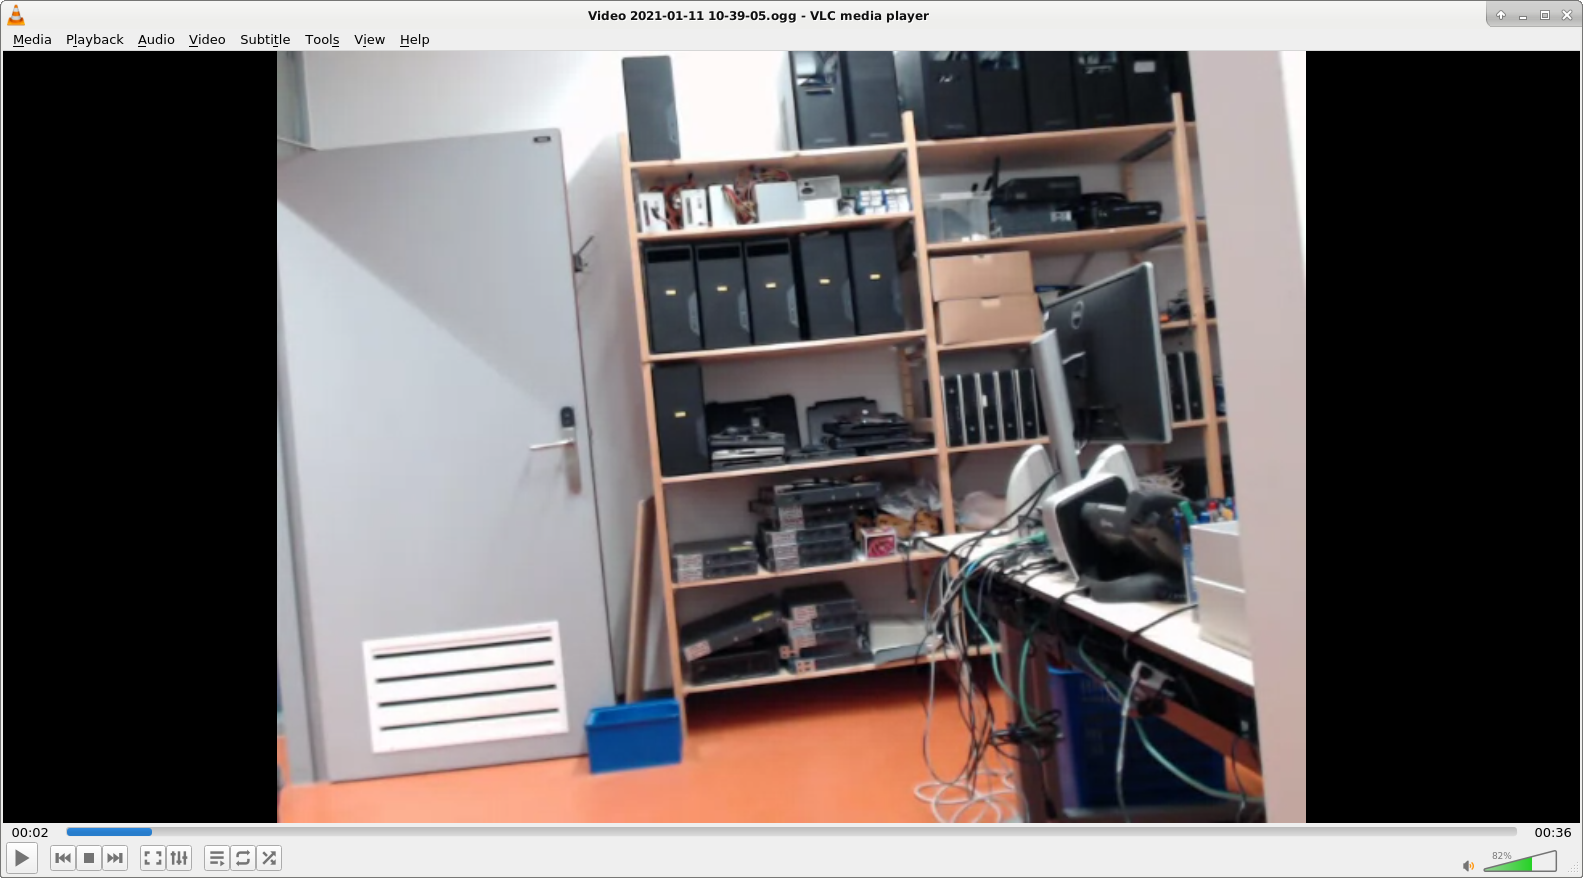
\includegraphics[]{VLC-working.png}
\caption{VLC}
\end{figure}
\end{center}
